\documentclass[12pt]{article}

\usepackage[utf8]{inputenc}
\usepackage[portuguese]{babel}
\usepackage{indentfirst}
\usepackage{amsmath}
\usepackage{hyperref}
\usepackage[numbers,super]{natbib}
\usepackage{graphicx}
\usepackage{geometry}

\geometry{
	paper = a4paper,
    inner = 3cm,
    outer = 3cm,
    bindingoffset = .5cm,
    top = 2cm,
    bottom = 2cm
}

\begin{document}

% Title page
\begin{titlepage}
\begin{center}

\textbf{\LARGE Universidade Federal de Alagoas } \\[0.5cm]
\textbf{\large Instituto de Computação - IC}\\[0.2cm]

\vspace{20pt}

\vspace{20pt}
\vspace{20pt}
\vspace{20pt}
\vspace{20pt}
\vspace{20pt}
\vspace{20pt}
\vspace{20pt}
\vspace{20pt}

\textbf{\Large Aluno: Danilo Fernandes Costa}\\
\vspace{70pt}
\textbf{\LARGE Relatório de acopanhamento de pesquisa}\\
\vspace{20pt}
\textbf{\Large Análise e processamento de imagens PolSAR}\\
\vspace{70pt}
\textbf{\large Orientador: Alejandro Frery}\\

\vspace{45pt}
\end{center}

\par
\vfill
\begin{center}
\textbf{Maceió - AL}\\
\textbf{2018}
\end{center}

\end{titlepage}

\newpage

\section{Resumo}

O presente relatório apresenta algoritmos implementados em R para visualização de imagens PolSAR provenientes de arquivos dos tipos MLC (\textit{calibrated multi-looked cross products}) e SLC (\textit{calibrated single look complex}) utilizando a biblioteca raster. Tais implementações projetam diretamente matrizes de covariância no espaço das cores e utilizam as funcionalidades dessa biblioteca para processar os dados referentes as imagens sem carregá-los de uma única vez na memória.

Nessa abordagem, a função de distribuição acumulada empírica, a qual é essencial para a equalização dos dados, é definida a partir de amostras extraídas destes. A justificativa para isto é que não foi encontrada uma implementação dessa função na bilioteca raster e a nativa do R requer que os dados destinados a sua definição estejam na memória principal.

Para obtenção das amostras foram empregadas a amostragem aleatória simples e a estratificada, as quais foram implementadas de forma independente para fins comparativos. Dessa forma, obtemos duas subabordagens para visualização do dado PolSAR, as quais foram comparadas por meio do cálculo de erro médio entre as matrizes equalizadas obtidas por cada subabordagem em relação àquelas obtidas pelo algoritmo descrito no relatório anterior.

\section{Nova abordagem para visualização de imagens PolSAR}

Uma característica de grande relevância da biblioteca raster é permitir criar objetos associados a arquivos no disco rígido e fornecer funcionalidades para manipulação dos dados contidos nestes sem precisar mantê-los, em totalidade, na memória principal.

O formato padrão Raster para esses tipos de arquivos consiste em um arquivo de texto com metadados e outro binário com dados. Além disso, ambos devem apresentar mesmo nome, diferindo apenas na extensão, onde no primeiro será .grd e o segundo, .gri. Para associar um arquivo MLC a um objeto Raster é necessário, inicialmente, mudar a extensão do mesmo para .gri e criar um arquivo de metadados para ele. Isto é feito pelas instruções a seguir:

\begin{verbatim}

intensity_band <- raster(nrow = nrows, ncol = ncols)
hdr(intensity_band, format = "RASTER", filename = "<filename>.grd")
intensity_band <- raster("<filename>.grd")

\end{verbatim}

A primeira linha cria um objeto Raster com as dimensões da imagem PolSAR, o qual existirá na memória apenas como um objeto de metadados. A segunda cria o arquivo .grd e neste haverá informações sobre o arquivo binário ao qual estará associado como ordem dos \textit{bytes} e o tipo dos dados; os quais, neste caso, serão \textit{little endian} e valor com ponto flutuante representado em 4 \textit{bytes}. Já a última linha carregará o dado PolSAR em um objeto Raster.

Para extrair as amostras do objeto Raster por meio de amostragem aleatória simples, executa-se a instrução a seguir:

\begin{verbatim}
sample_intensity_band <- sampleRandom(intensity_band, sample_size)
\end{verbatim}

O parâmetro \texttt{sample\textunderscore size} é o tamanho da amostra; a qual, nesta implementação, foi estabelecida como o número de \textit{pixels} da imagem divido por dois mil. É fácil notar que esse método de amostragem não dá garantias de que as amostras serão elementos que se encontram bem distribuídos em uma matriz que venha a representar uma banda de intensidade. 

Uma maneira de obter aproximadamente a mesma quantidade de amostras e melhor distribuídas é dividindo cada matriz de intensidade em um conjunto de submatrizes, as quais podem ser pensadas como estratos, e de cada uma destas extrair uma amostra aletória simples. No entanto, não existe uma função na biblioteca raster que realize essa tarefa. Por esse motivo foi necessário implementar a função mySampleStratified para que o fizesse. Essa função recebe um objeto Raster e o número de células por estrato, cujo valor nessa implementação foi estipulado como dois mil, e retorna as amostras. Segue a sua assinatura:

\begin{verbatim}
sample_intensity_band<-mySampleStratified(intensity_band,
                                         stractum_size)
\end{verbatim}

Em sua implementação define-se as submatrizes como quadradas, cujas dimensões são a iguais a raiz quadrada de \texttt{stractum}\textunderscore\texttt{size}. Segue a sua implementação:

\begin{verbatim}
mySampleStratified <- function(raster_obj, stractum_size){
  
  dim_stractum <- floor( sqrt(stractum_size) )
  
  range_i <- floor( nrow(raster_obj) / dim_stractum )
  range_j <- floor( ncol(raster_obj) / dim_stractum )
  
  sample <- array(length(range_i*range_j))
  count <- 0
  
  for(i in 1:range_i){
    for(j in 1:range_j){
     
      sample[count] <- raster_obj[(i-1)*dim_stractum 
      + sample(1:dim_stractum, 1), (j-1)*dim_stractum
      + sample(1:dim_stractum, 1)]
      
      count <- count + 1  
    }
  }
  return(sample)
}
\end{verbatim}

Em posse do conjunto de amostras; pode-se estabelecer a função de distribuição acumulada empírica, a partir deste, através da seguinte instrução:

\begin{verbatim}
empirical_distribution <- ecdf(sample_intensity_band)
\end{verbatim}

Contudo, para aplicá-la aos dados, o que seria o processo de equalização, foi utilizada a função \texttt{calc} da biblioteca raster. Essa aplica uma dada função a todos dados de um objeto Raster, mantendo em memória somente uma parte dos mesmos e que ainda não foram processados. Segue a instrução de equalização:

\begin{verbatim}
equalized_intensity_band <- calc(intensity_band,
empirical_ditribution, filename = "equal_insensity_band.grd")
\end{verbatim}

Deve ser observado que \texttt{calc} criará um arquivo no padrão Raster com o resultado da aplicação de \texttt{empirical}\textunderscore \texttt{distribution} a \texttt{intensity}\textunderscore\texttt{band} e retornará um objeto Raster associado a esse arquivo.

Após os procedimentos acima serem realizados para as três bandas de intensidade, pode-se, finalmente, gerar a imagem. A implementação desenvolvida visou gerar a imagem por blocos e posteriormente agrupá-los utilizando recursos de outras bibliotecas de processamento de imagens. Essa perspectiva permite gerar grandes imagens usando os recursos de memória de forma eficiente. 

Para extrair de um RasterLayer  -- objeto Raster com o qual tem-se trabalhado nesta implementação -- um bloco de dados no formato de matriz, executa-se o seguite:

\begin{verbatim}
intensities_matrix[,,i] <- getValuesBlock(
                              equalized_intensity_band,
                              nrow = 1, nrows = num_rows,
                              ncol = 1, ncols = num_cols,
                              format = "matrix")

\end{verbatim}

Deve ser observado que \texttt{intensities}\textunderscore\texttt{matrix} é a matriz de ordem \texttt{num}\textunderscore\texttt{cols} x \texttt{num}\textunderscore\texttt{rows} x 3 que conterá as bandas RGB e i que varia de 1 a 3. A ordem com que as matrizes equalizadas que representam as bandas de intensidades irão se dispor em \texttt{intensities}\textunderscore\texttt{matrix} é a mesma que a apresentada para a projeção direta no espaço das cores no relatório anterior. 

Para gerar a imagem referente a \texttt{intensities}\textunderscore\texttt{matrix}, executa-se:

\begin{verbatim}
writePNG(intensities_matrix, target = "image.png")
\end{verbatim}

Aplicou-se as abordagens que empregam amostragem aletória simples e estratificada a duas imagens PolSAR diferentes provenientes de dados MLC obtidos em UAVSAR. Seguem os resultados obtidos da primeira imagem, a qual trata-se de a um região de \href{https://uavsar.jpl.nasa.gov/cgi-bin/product.pl?jobName=evergl_26301_10053_003_100622_L090_CX_01#data}{Everglades, Florida, EUA}:\\

\begin{figure}[!ht]
	\begin{center}
		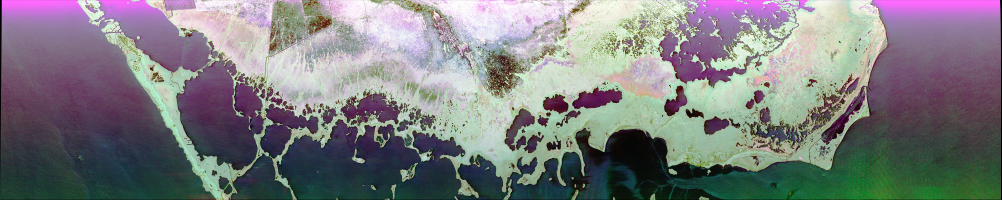
\includegraphics[width = 150mm, scale = 0.5]{../../Images/Report_08_18/florida_simple_random_sample_reduced} \\ 
        Amostragem aleatória simples\\
	\end{center}
\end{figure}

\newpage

\begin{figure}[!ht]
	\begin{center}
		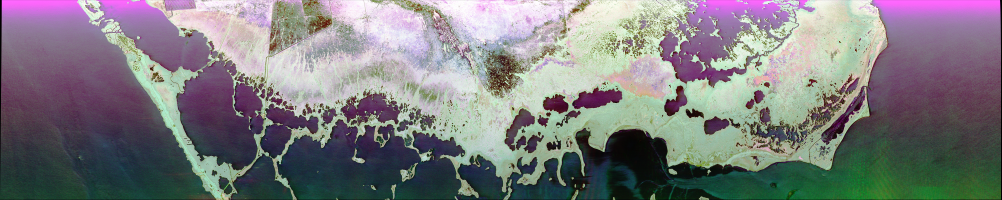
\includegraphics[width = 150mm, scale = 0.5]{../../Images/Report_08_18/florida_stratified_sample_reduced} \\ 
        Amostragem estratificada\\
	\end{center}
\end{figure}

\begin{figure}[!ht]
	\begin{center}    
		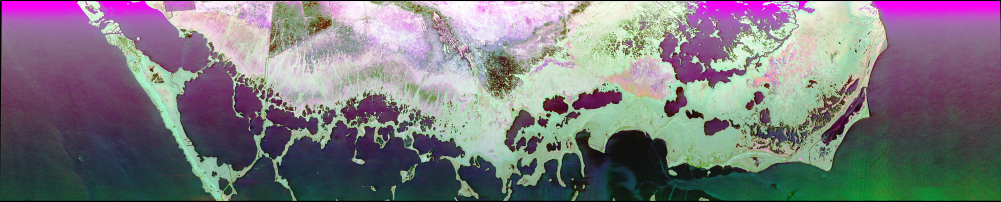
\includegraphics[width = 150mm, scale = 0.5]{../../Images/Report_08_18/florida_trad_algorithm} \\ 
        Antigo algoritmo\\
	\end{center}
\end{figure}

Seguem os resultados obtidos da segunda imagem, que é uma região de \href{https://uavsar.jpl.nasa.gov/cgi-bin/product.pl?jobName=trauns_22551_15087_016_150604_L090_CX_01#data}{Traunstein, Bayern, Alemanha}:

\begin{figure}[!ht]
	\begin{center}
        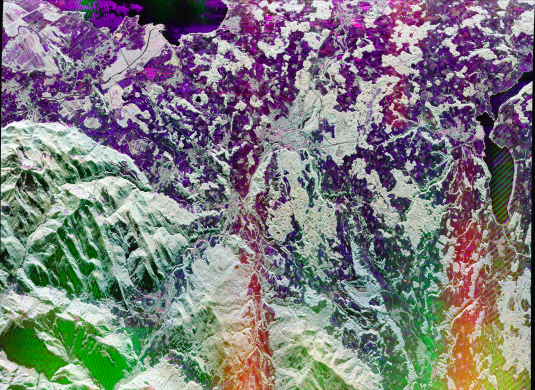
\includegraphics[width = 120mm, scale = 0.5]{../../Images/Report_08_18/traunstein_simple_random_sample_reduced} \\ 
        Amostragem aleatória simples\\
	\end{center}
\end{figure}

\begin{figure}[!ht]
	\begin{center}
		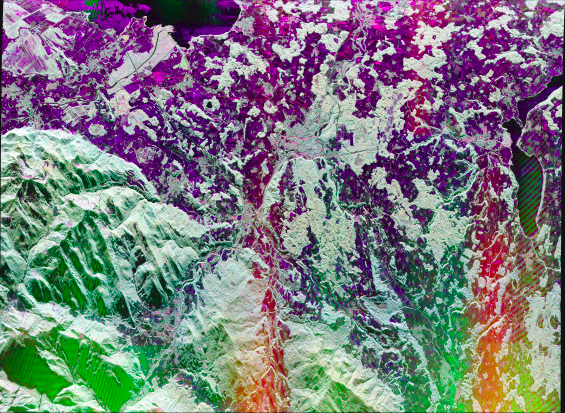
\includegraphics[width = 120mm, scale = 0.5]{../../Images/Report_08_18/traunstein_stratified_sample_reduced} \\ 
        Amostragem estratificada\\
	\end{center}
\end{figure}

\begin{figure}[!ht]
	\begin{center}    
		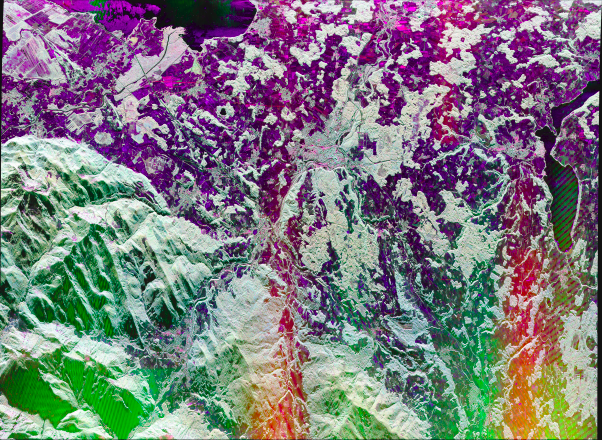
\includegraphics[width = 120mm, scale = 0.5]{../../Images/Report_08_18/traunstein_trad_algorithm_reduced} \\ 
        Antigo algoritmo\\
	\end{center}
\end{figure}

\newpage

O processo para obtenção de imagens provenientes de arquivos SLC diferirá do descrito acima apenas por um processamento prévio para a geração dos dados referentes às bandas de intensidades. Isso se deve ao fato de que cada um desses arquivos contém valores complexos correspondentes aos sinais medidos pelo dispositivo imageador em uma dada polarização. Cada um desses valores está associado a um pixel da imagem e cuja intensidade, nessa polarização, é o quadrado do módulo desse valor complexo.

Tal processamento é realizado pela seguinte função, a qual recebe um arquivo binário com os valores complexos referentes a uma dada polarização, as dimensões da imagem e o nome do arquivo de destino.

\begin{verbatim}
generate_intensity_file <- function(file, nrow, ncol, tag){
  
  file_amp <- file(tag, "wb")
  
  remain <- 2*nrow * ncol
  default <- 10000000
  
  while(remain > 0){
    
    elements_to_read <- min(remain, default)
    complex_numbers <- matrix(
      readBin(file, double(), n = elements_to_read, size = 4,
              endian = "little"), 
      nrow = nrow*ncol, ncol = 2, byrow = TRUE) 
    
    writeBin(complex_numbers[,1]^2 + complex_numbers[,1]^2, file_amp,
             size = 4, endian = "little", useBytes = FALSE)
    
    rm(complex_numbers)
    remain <- remain - elements_to_read
    
  }
  
  close(file_amp)
  
}
\end{verbatim}

Devem ser observados dois detalhes na implementação acima. O primeiro é que os dados do arquivo binário são lidos e processados por partes, para evitar a exaustão da memória. Já o segundo é sobre o fato de que o valor complexo no arquivo binário é armazenado como um par de valores de ponto flutante, onde o primeiro é a parte a real e o segundo, a imaginária. Além disso cada um deles é representado em quatro \textit{bytes}.

Seguem os resultado obtidos a partir de dados SLC de uma de região de \href{https://earth.esa.int/web/polsarpro/data-sources/sample-datasets#ESAR}{Oberpfaffenhofen, Alemanha}:

\begin{figure}[!ht]
	\begin{center}
        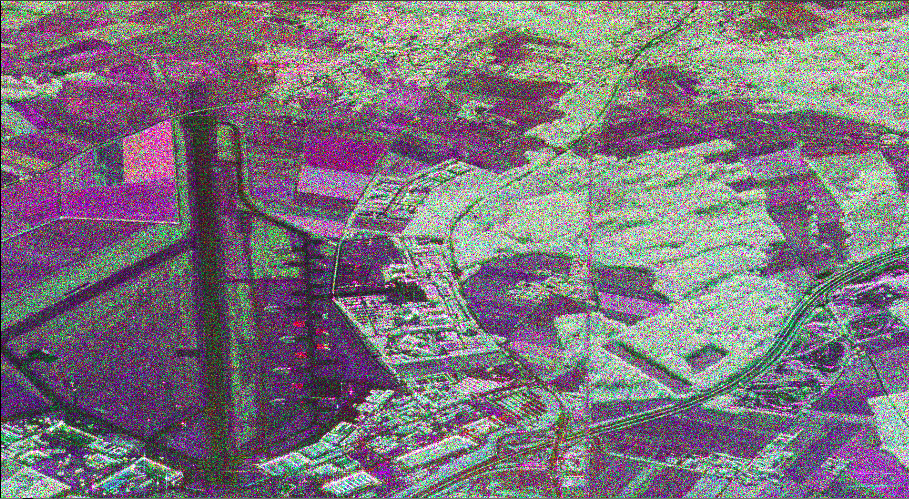
\includegraphics[width = 98.5mm, scale = 0.5]{../../Images/Report_08_18/oberpfaffenhofen_simple_random_sample_reduced} \\ 
        Amostragem aleatória simples\\
	\end{center}
\end{figure}

\begin{figure}[!ht]
	\begin{center}    
		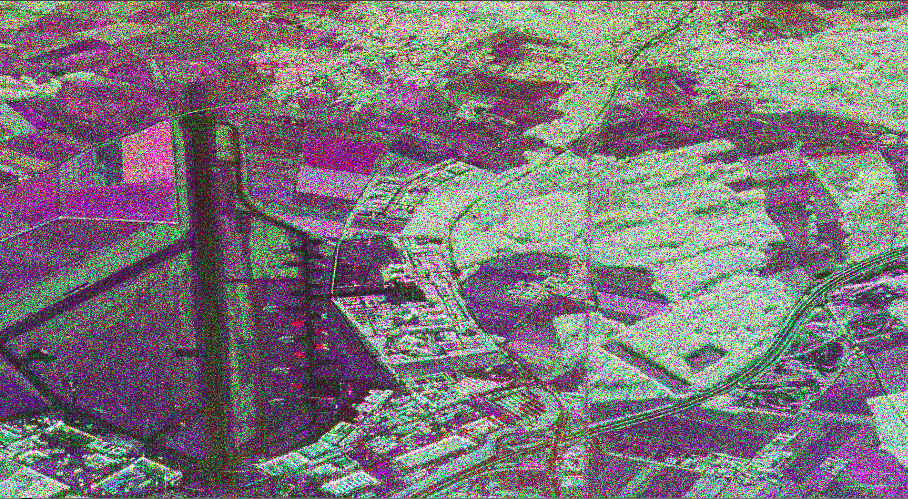
\includegraphics[width = 98.5mm, scale = 0.5]{../../Images/Report_08_18/oberpfaffenhofen_trad_algorithm_reduced} \\ 
        Antigo algoritmo\\
	\end{center}
\end{figure}

\newpage

\section{Calculo do erro médio}

Para obter valores quantitativos que descrevessem a divergência entre os resultados dessa abordagem em relação àquela feita no relatório anterior, calculou-se o erro médio das imagens visualizadas provenientes de dados MLC. O erro médio foi assumido como a soma dos módulos das diferenças entre as células correspondentes de duas matrizes equalizadas, onde uma foi pelo algoritmo antigo, dividida pelo número de células de uma das matrizes.

Observou-se que o erro médio para uma matriz equalizada utilizando a subabordagem de amostragem aleatória simples foi, em média, de 0.00343695533. Já para aquela que utilizou amostragem estratificada, esse erro foi, em média, 0.00199967765.

Calculou-se também esse erro quando função \texttt{ecdf} é definida a partir de todos os dados e aplicada a eles por meio da função \texttt{calc}. Este foi, em média, $9.934892333 \cdot 10^{-9}$.

%Referências bibliograficas
%\bibliographystyle{unsrt}
%\bibliography{Bibliography/ref}

\end{document}
